\documentclass[a4paper,latin,center,twocolumn]{paper} 
\usepackage[english]{babel}
\usepackage{hyperref}

\usepackage[margin=2.5cm]{geometry}
\usepackage{graphicx}
\usepackage{lipsum}
\usepackage{xcolor}
\usepackage{booktabs}

\sectionfont{\large\sf\bfseries\color{black!60!blue}} 
\subsectionfont{\normalsize\sf\bfseries}

\title{ME748: Computer Aided Simulation of Machines}

\subtitle{Term Project 2: Static and Dynamic Analysis \\
\hfill
\includegraphics[height=2cm]{Images/Indian_Institute_of_Technology_Bombay_Logo.png}
\vspace{-2cm}}

\author{Madhav Joshi, Roll No - 190110034} 
\institution{Indian Institute of Technology Bombay}

\begin{document}
    \selectlanguage{english}
    % \twocolumn[\maketitle 
    %     \hrule 
    %     \bigskip
    % ]
    \onecolumn\maketitle 
    \hrule 
    \bigskip

    \begin{abstract}
    Here, the (virtual) model created in Term Project 1 is used to perform a static force analysis and verify the results by manual computation. Then perform a dynamic motion analysis for varying force/torque profiles.
\end{abstract}


    \smalltableofcontents

    \section{Static Force Analysis} 
    A constant force (in a constant global direction) should be applied to a specific point of the output component and the force/torque needed at the driving component to keep/hold the mechanism in this position under this condition needs to be obtained from the software. This should be done with the mechanism in four positions, preferably the same four positions which were used for theoretical evaluation of kinematic parameters in Term Project 1. The point and direction of application of this force should be shown in four snapshots.

    \begin{enumerate}
        \item Position 1 
            \begin{figure}[hbt!]
                \centering
                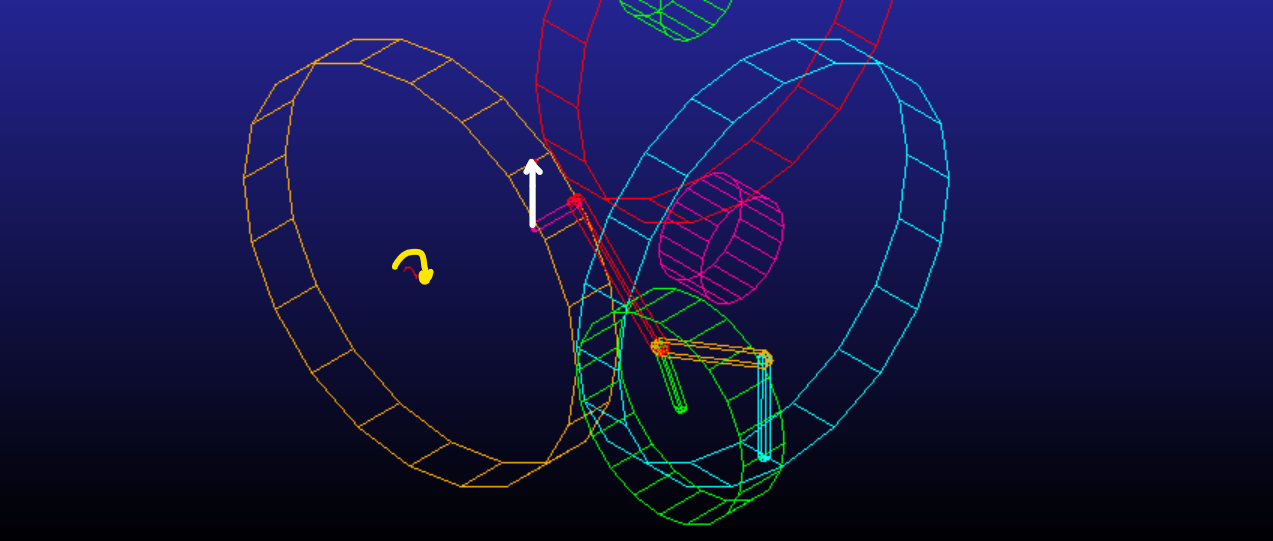
\includegraphics[width=0.9\columnwidth]{Images/Force_pos0.png}
                \caption{Mechanism and Force applied}
                \label{fig:force_applied}
            \end{figure}
            In fig~\ref{fig:force_applied}, the white arrow indicates the force applied on the output link whose magnitude is 50 kg-mm/s\^2. And the yellow curved arrow indicates the torque applied to prevent the system from moving which comes out to be -5500 kg-mm\^2/s\^2.
            \begin{figure}[hbt!]
                \centering
                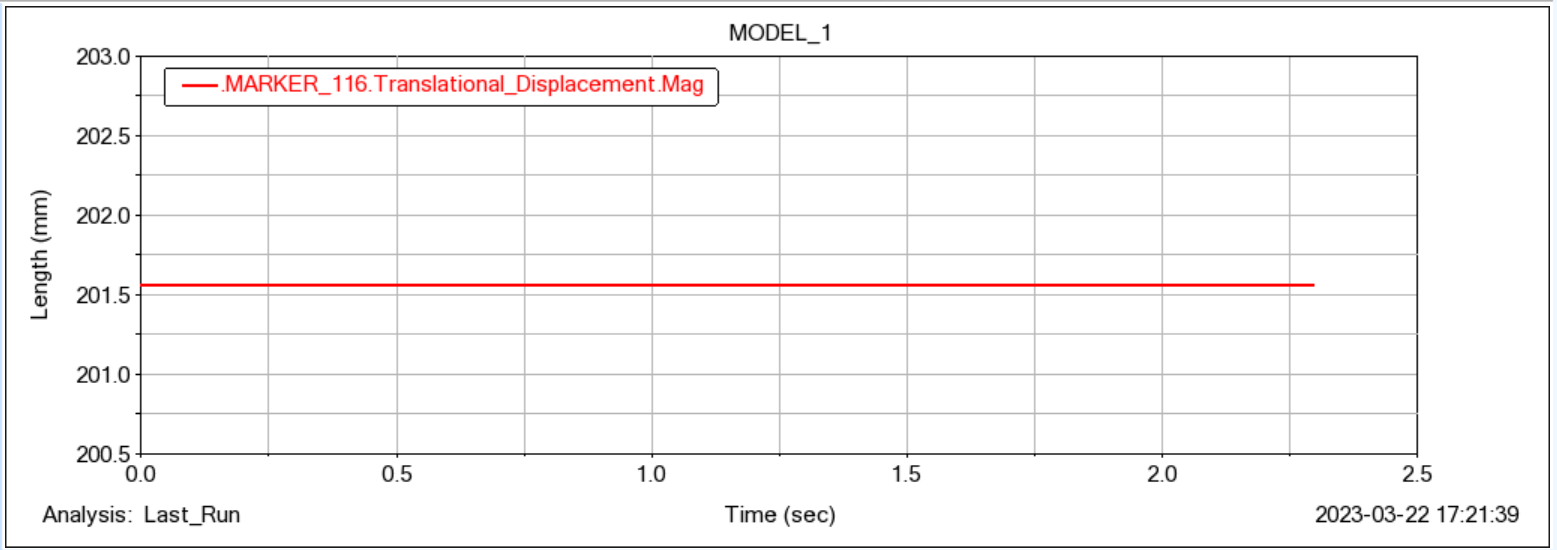
\includegraphics[width=0.9\columnwidth]{Images/Steady_output.png}
                \caption{Output displacement vs time}
                \label{fig:steady_out}
            \end{figure}
            Output displacement plot is shown in fig~\ref{fig:steady_out}, which is constant that indicates the applied torque at the input gear prevents the output link from moving.
            
            % \begin{verbatim}
            %     your
            %     code
            %     example
            % \end{verbatim}
    \end{enumerate}
            

    \section{Validation of static force analysis} 
    A manual validation of the static force analysis for any one of the values reported in Section 1. See fig 3 and fig 4.
    \begin{figure}[hbt!]
        \centering
        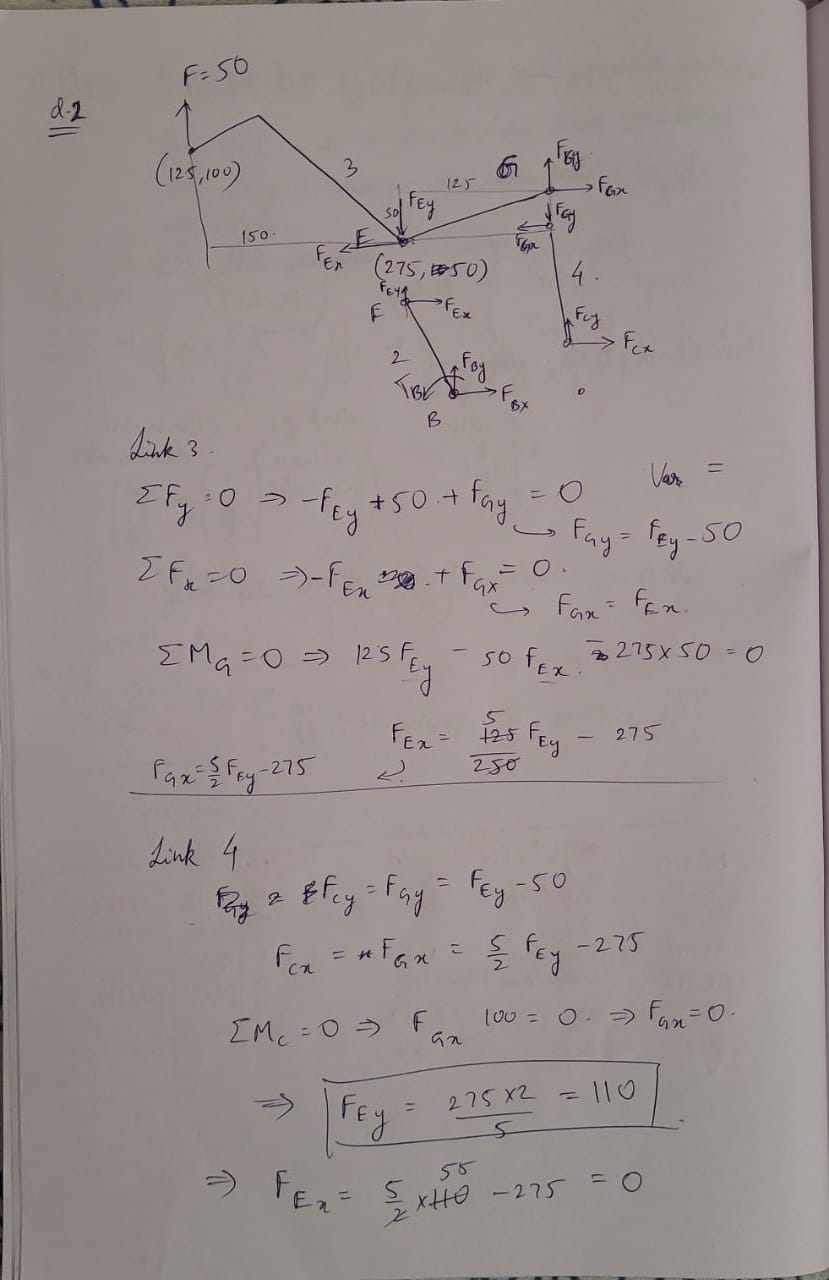
\includegraphics[width=0.9\columnwidth]{Images/proof1.jpeg}
        \caption{page1}
        \label{fig:page1}
    \end{figure}
    \begin{figure}[hbt!]
        \centering
        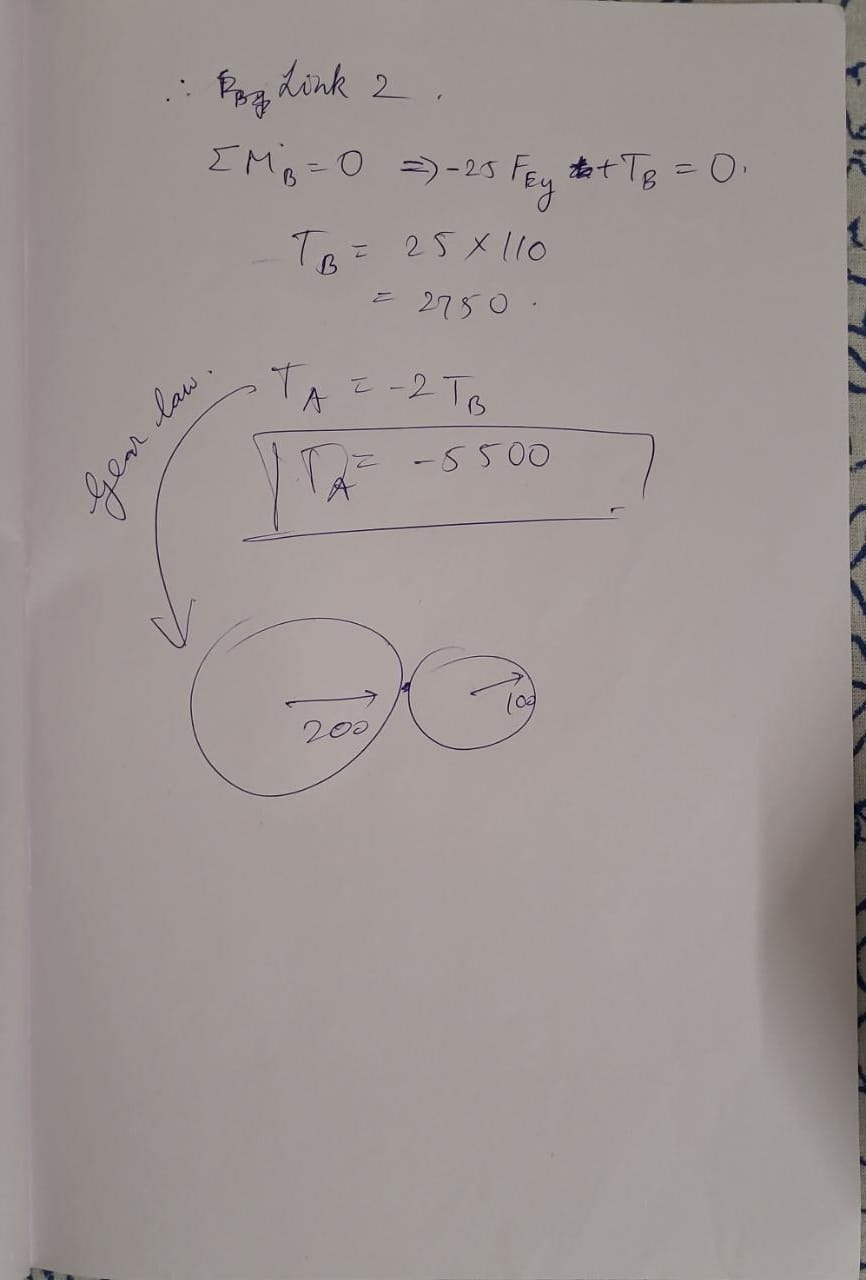
\includegraphics[width=0.9\columnwidth]{Images/proof2.jpeg}
        \caption{page2}
        \label{fig:page2}
    \end{figure}

    \section{Dynamic motion analysis}
    \subsection{Constant driving force/torque}
        \subsubsection{Velocity and Acceleration}
            Providing a constant input torque of 5500 kg-mm\^2/s\^2 clockwise.
            \begin{enumerate}
                \item 
                    \begin{figure}[hbt!]
                        \centering
                        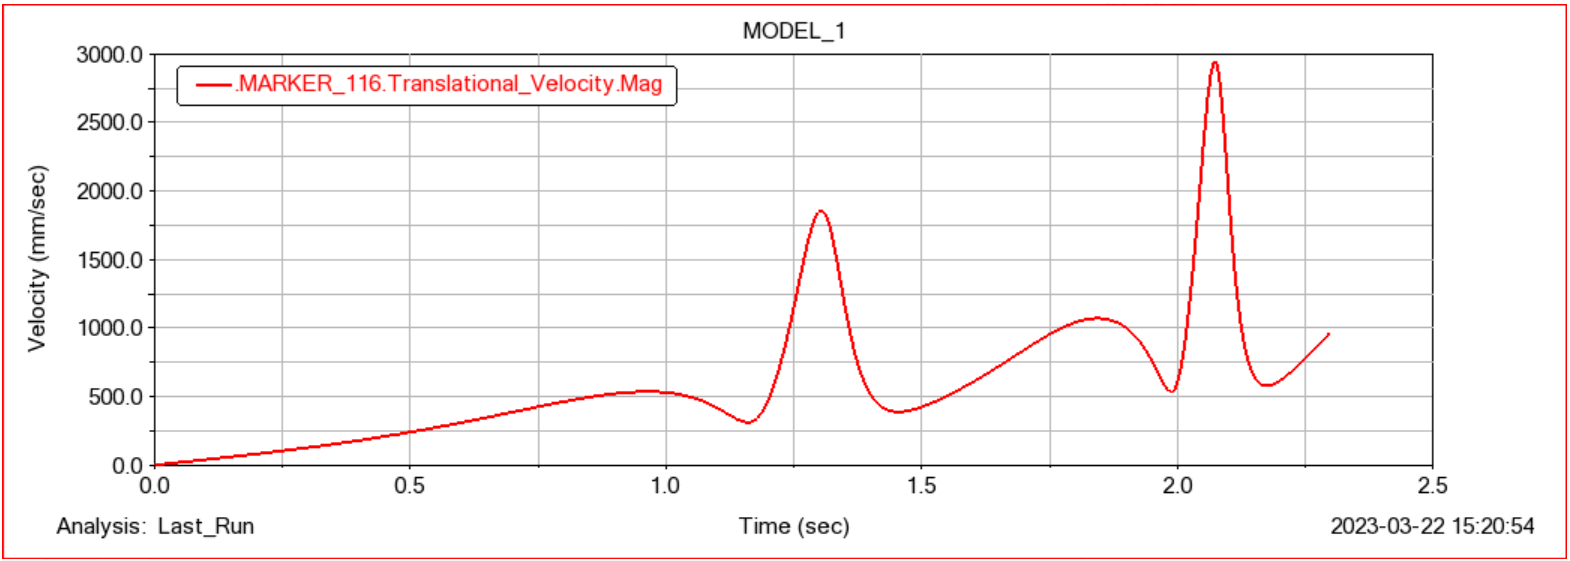
\includegraphics[width=0.9\columnwidth]{Images/Velocity_311.png}
                        \caption{Velocity vs time}
                        \label{fig:vel_1}
                    \end{figure}
                    Velocity plot is shown in fig~\ref{fig:vel_1}
                \item 
                    \begin{figure}[hbt!]
                        \centering
                        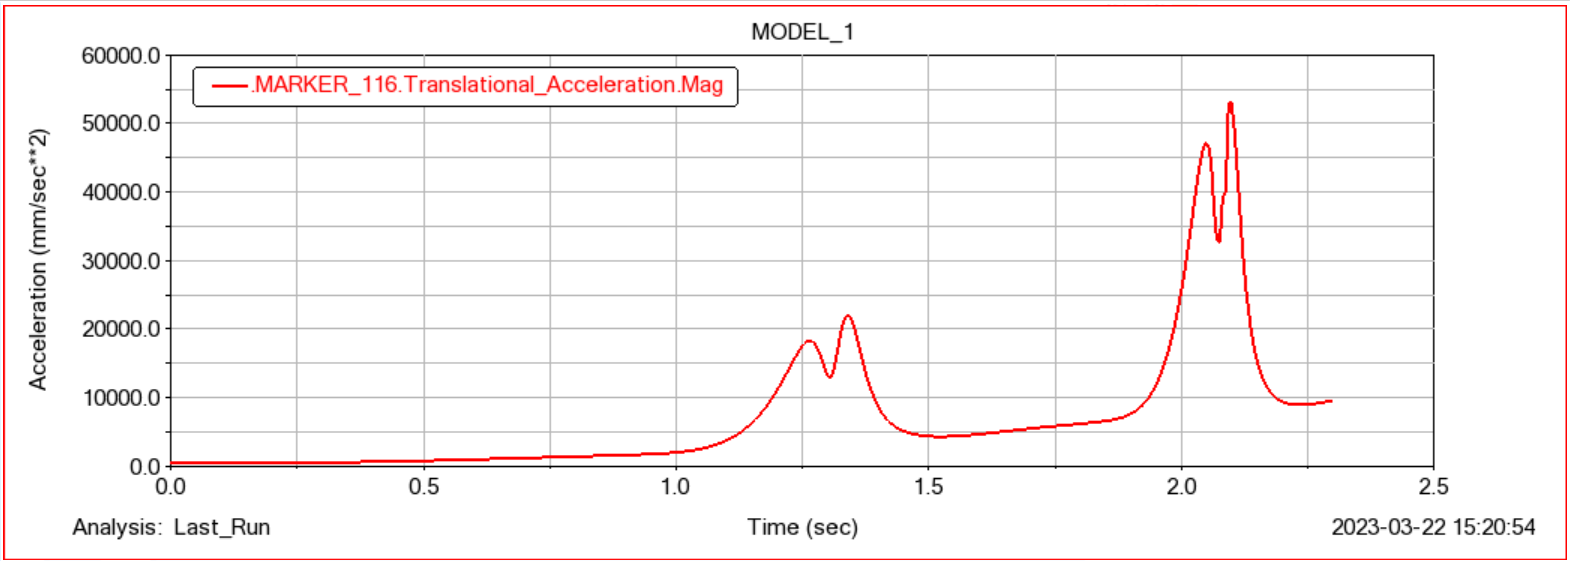
\includegraphics[width=0.9\columnwidth]{Images/Acceleration_311.png}
                        \caption{Acceleration vs time}
                        \label{fig:acc_1}
                    \end{figure}
                    Acceleration plot is shown in fig~\ref{fig:acc_1}
            \end{enumerate}
        \subsubsection{Sub2}
            Applying twice the torque applied in previous section i.e. -11000 kg-mm\^2/s\^2. Superimposed plots are shown below.
            \begin{enumerate}
                \item 
                    \begin{figure}[hbt!]
                        \centering
                        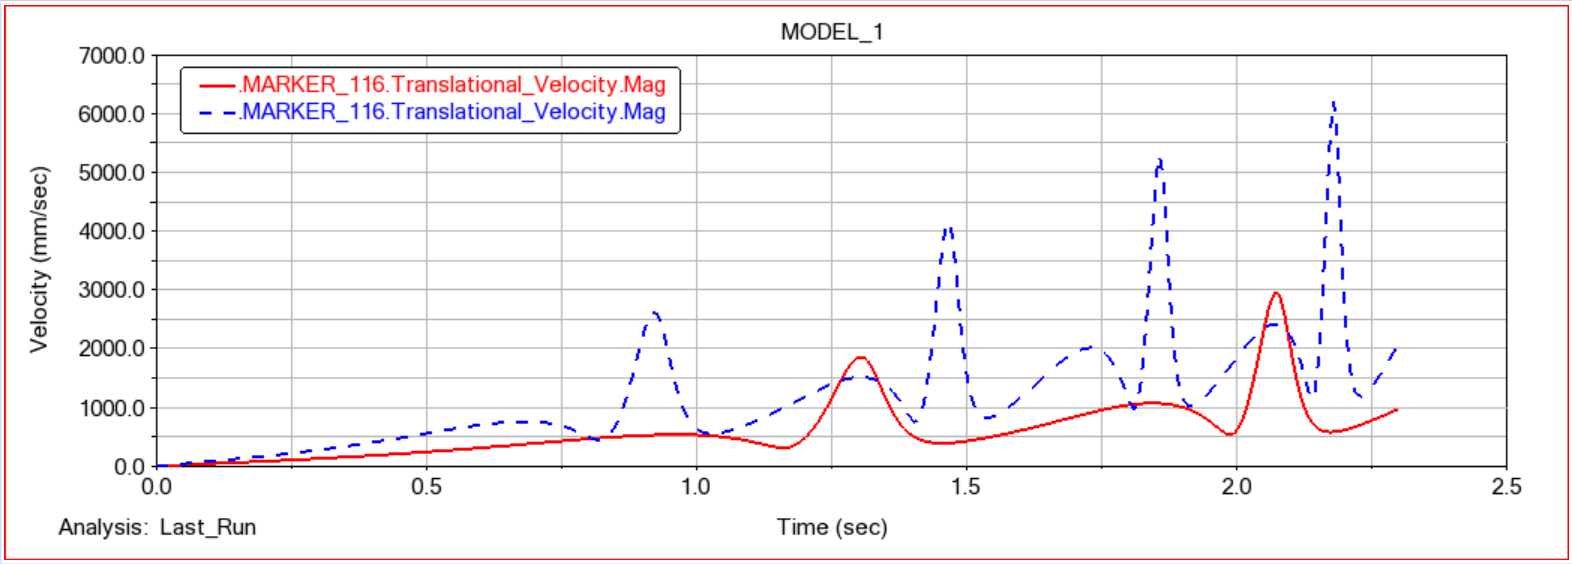
\includegraphics[width=0.9\columnwidth]{Images/Velocity_312.png}
                        \caption{Superimposed velocity vs time}
                        \label{fig:vel_2}
                    \end{figure}
                    Velocity plot is show in fig~\ref{fig:vel_2}
                \item 
                    \begin{figure}[hbt!]
                        \centering
                        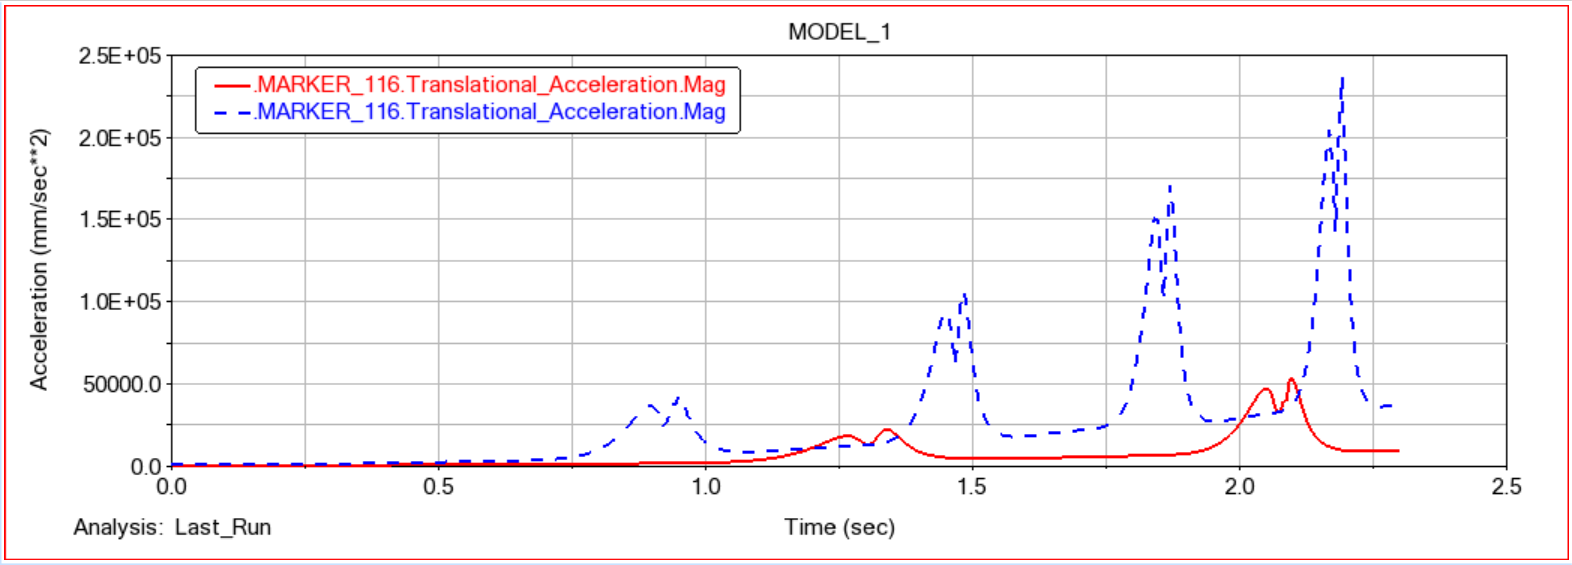
\includegraphics[width=0.9\columnwidth]{Images/Acceleration_312.png}
                        \caption{Superimposed acceleration vs time}
                        \label{fig:acc_2}
                    \end{figure}
                    Acceleration plot is shown in fig~\ref{fig:acc_2}
            \end{enumerate}
            
    \subsection{Sinusoidal driving force/torque}
        Now we apply sinusoidal torque $T = 1.4*5500*(1+\sin(40t))$.
        \begin{figure}[hbt!]
            \centering
            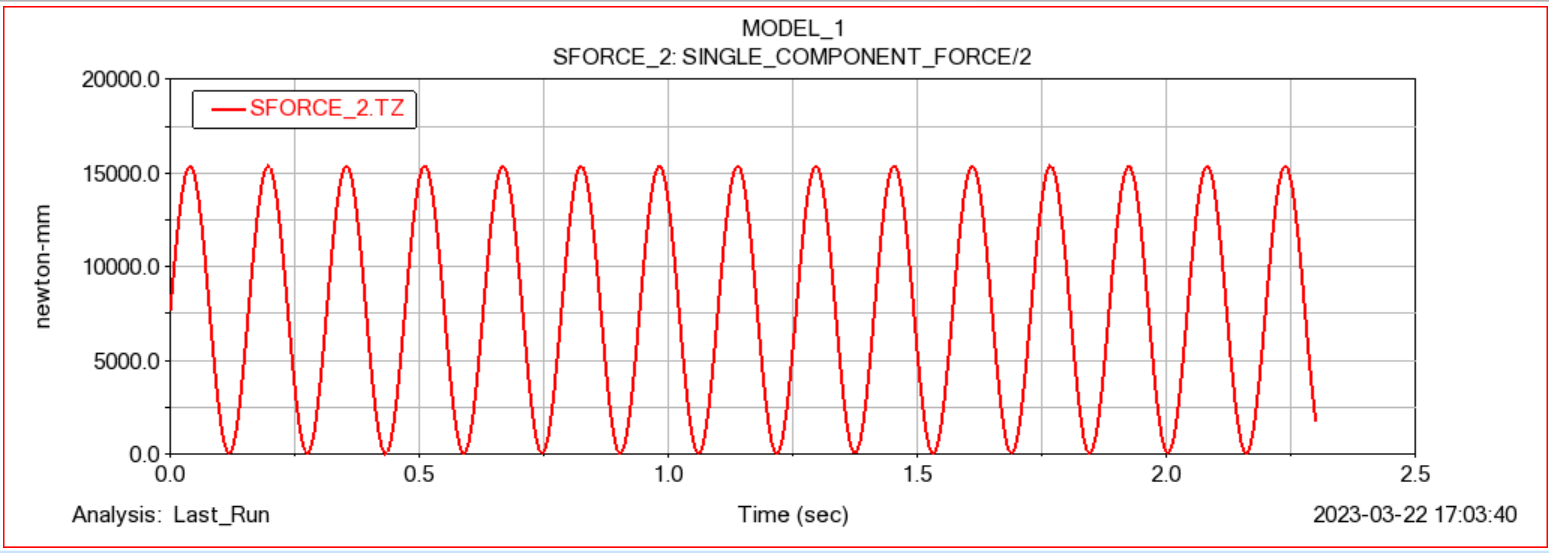
\includegraphics[width=0.9\columnwidth]{Images/Force_sinusoidal.png}
            \caption{Sinusoidal force vs time}
            \label{fig:sin_force}
        \end{figure}
        The force graph has been shown in fig~\ref{fig:sin_force}.
        \begin{enumerate}
            \item 
                \begin{figure}[hbt!]
                    \centering
                    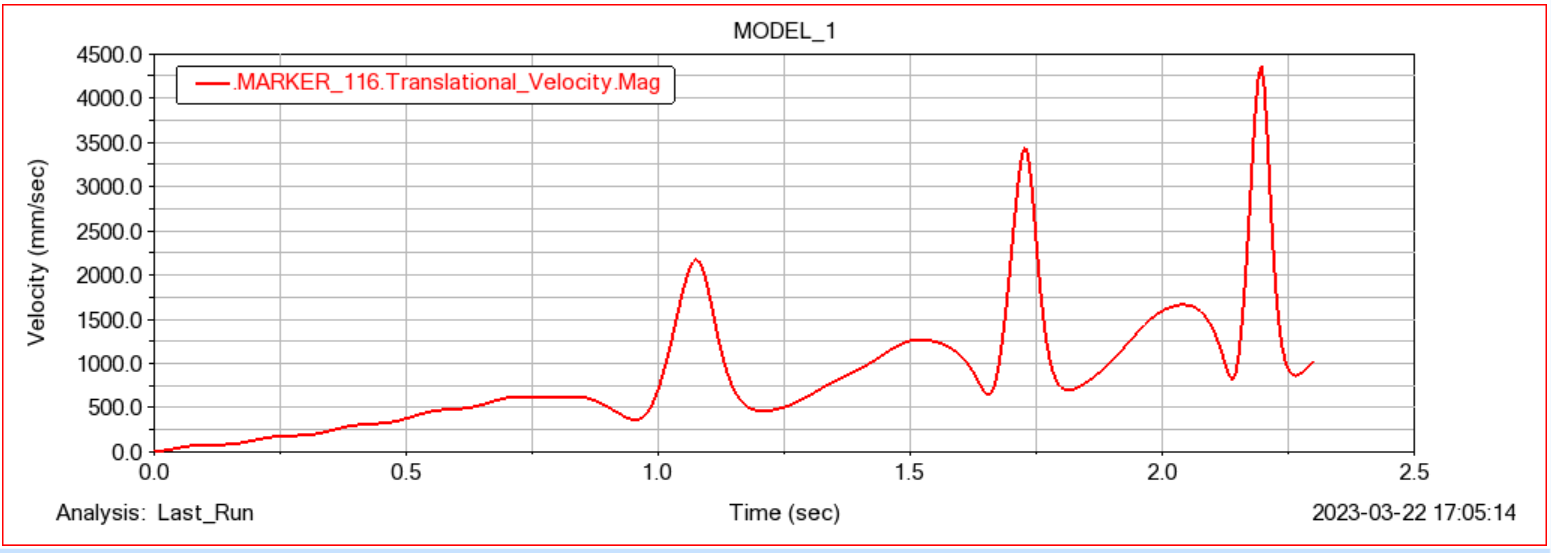
\includegraphics[width=0.9\columnwidth]{Images/sine_vel.png}
                    \caption{Velocity for sine force vs time}
                    \label{fig:sine_vel}
                \end{figure}
                Velocity plot is shown in fig~\ref{fig:sine_vel}
            \item 
                \begin{figure}[hbt!]
                    \centering
                    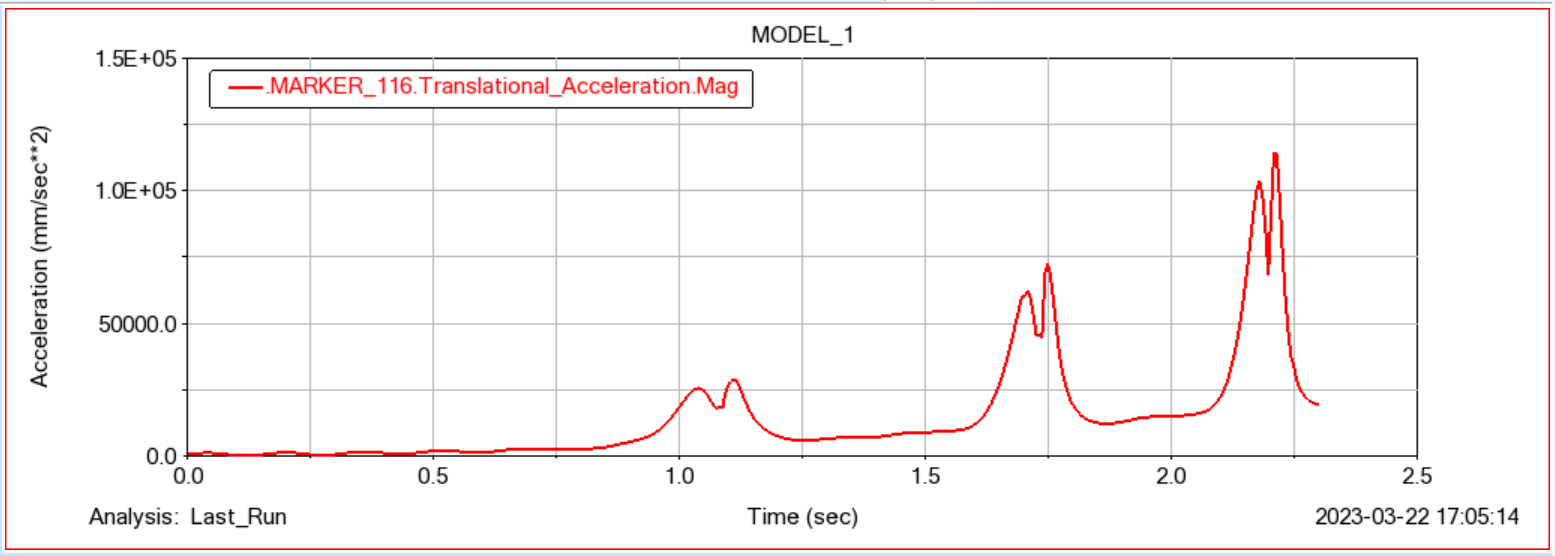
\includegraphics[width=0.9\columnwidth]{Images/sine_acc.png}
                    \caption{Acceleration for sine force vs time}
                    \label{fig:sine_acc}
                \end{figure}
                Acceleration plot is shown in fig~\ref{fig:sine_acc}
        \end{enumerate}

    \begin{thebibliography}{999}

    \bibitem{camPST}
        Liang Sun, Xuan Chen, Chuanyu Wu, Guofeng Zhang, Yadan Xu, 
        \emph{Synthesis and design of rice pot seedling transplanting mechanism based on labeled graph theory},
        Computers and Electronics in Agriculture,
        Vol. 143,
        2017,
        Pages 249-261,
        ISSN 0168-1699,
        \href{https://doi.org/10.1016/j.compag.2017.10.021}{https://doi.org/10.1016/j.compag.2017.10.021}
        
    \bibitem{6rowManuallyOperatedTransplanter}
        Yadav, Dr \& Mital, Patel \& P, Shukla \& Pund, Sahastrarashmi. (2007). \emph{Ergonomic evaluation of manually operated six-row paddy transplanter.} International Agricultural Engineering Journal. 16. 147-157. 
    
    \bibitem{selfPropelled}
        Guru, Prabhat \& Chhuneja, Naresh \& Dixit, Anoop \& Tiwari, Prem \& Kumar, Anjani. (2018). \emph{Mechanical transplanting of rice in India: Status, technological gaps and future thrust.} ORYZA- An International Journal on Rice. 55. 10.5958/2249-5266.2018.00012.7. 
    
\end{thebibliography}

\end{document}